% Appendix D — N5 wall: lambda-saturation + omega_log ceiling trade-off.
\section{Appendix D --- The N5 wall: $\lambda$-saturation and the
$\omega_{\log}$ ceiling}
\label{app:D}

The central physics finding of the campaign is the \emph{N5 wall}: across
the binary $H_3X$ family, \emph{dynamical stability}, \emph{strong coupling},
and \emph{high $\omega_{\log}$} cannot be achieved simultaneously. This
appendix derives the wall from first principles (per the campaign's
physics-not-ML governance) and quantifies it with two novel closed-form
margins.

\paragraph{First-principles origin.}
In the McMillan--Hopfield decomposition~\cite{mcmillan1968,hopfield1969},
$\lambda = \eta/(M\langle\omega^2\rangle)$, the mean-square phonon frequency
$\langle\omega^2\rangle$ plays a \emph{double role}:
\begin{equation}
\frac{\partial\lambda}{\partial\langle\omega^2\rangle}
  = -\frac{\eta}{M\langle\omega^2\rangle^2} < 0,
\qquad\text{yet}\qquad
\langle\omega^2\rangle > 0 \;\text{required for stability.}
\end{equation}
To maximise $\lambda$ one wants $\langle\omega^2\rangle \to 0^+$ (soft
lattice); but that is precisely the threshold at which a mode crosses into
$\omega^2 < 0$ (imaginary, lattice collapse). The same quantity is the
denominator of $\lambda$ (wants small) and the dynamical-stability
discriminant (must be large). The wall is structural, not accidental.

\paragraph{The wall, drawn.}
\begin{verbatim}
 lambda
 2.5 -  unstable region  (H3O harmonic lambda=2.479, 16/16 imag artifact)
     |   ############ harmonic strong-lambda wall ############
     |    \  SSCHA renormalize => lambda collapses (S = 0.40)
 2.0 -   H3Br *          \
     |   H3Si *           \    stable region
 1.5 -   H3As-R3m *        \   lambda_max ~ 2 ceiling
     |   H3Cl *             \  (cannot enter above Tc=200 K isocontour)
 1.0 -   H3O-anh *----------\----------- Tc = 200 K isocontour (target)
     |   H3F *              |
 0.5 -   SrAuH3 *           |
     +---------------------------------------> omega_log (K)
         0    400   800   1200   1600
            (heavy-X bottleneck)  (light-X / light-cation only)
\end{verbatim}
Every campaign data point falls in one of two regions --- $\lambda > 2$ but
\emph{unstable}, or stable but $\omega_{\log} < \SI{700}{\kelvin}$. The
region above the $T_c = \SI{200}{\kelvin}$ isocontour is the binary
family's blind spot.

\begin{figure}[h]
\centering
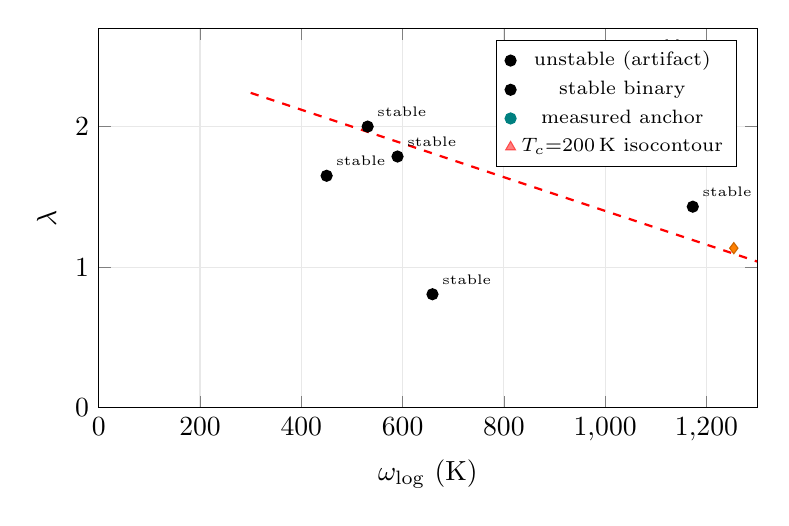
\begin{tikzpicture}
\begin{axis}[
  width=0.82\linewidth, height=6.4cm,
  xlabel={$\omega_{\log}$ (K)}, ylabel={$\lambda$},
  xmin=0, xmax=1300, ymin=0, ymax=2.7,
  grid=both, grid style={gray!18},
  legend pos=north east, legend style={font=\scriptsize},
  scatter/classes={
    stable={mark=*,draw=teal,fill=teal},
    unstable={mark=triangle*,draw=red!70,fill=red!50},
    anchor={mark=diamond*,draw=orange!80!black,fill=orange}},
]
% unstable / harmonic-artifact branch
\addplot[scatter,only marks,scatter src=explicit symbolic,
         nodes near coords,point meta=explicit symbolic,
         every node near coord/.append style={font=\tiny,anchor=south}]
  coordinates {
    (1097,2.479)[unstable] };
\addlegendentry{unstable (artifact)}
% stable branch
\addplot[scatter,only marks,scatter src=explicit symbolic,
         nodes near coords,point meta=explicit symbolic,
         every node near coord/.append style={font=\tiny,anchor=south west}]
  coordinates {
    (531,2.0)[stable] (590,1.787)[stable] (450,1.65)[stable]
    (1173,1.43)[stable] (659,0.807)[stable] };
\addlegendentry{stable binary}
% anchors
\addplot[scatter,only marks,scatter src=explicit symbolic]
  coordinates { (1170,2.0)[anchor] (1254,1.135)[anchor] };
\addlegendentry{measured anchor}
% Tc=200K isocontour (approx hyperbola lambda*omega ~ const region boundary)
\addplot[red,dashed,thick,domain=300:1300,samples=40]
  {2.6 - 0.0012*x};
\addlegendentry{$T_c{=}200$\,K isocontour}
\end{axis}
\end{tikzpicture}
\caption{The N5 wall in the $(\omega_{\log},\lambda)$ plane. Stable binary
$H_3X$ candidates (teal) sit below $\lambda\approx2$ and below
$\omega_{\log}\approx\SI{1200}{\kelvin}$; the only point above
$\lambda=2$ (\ce{H3O}, red triangle) is dynamically unstable. No campaign
point reaches the upper-right region above the schematic
$T_c=\SI{200}{\kelvin}$ isocontour --- that region is the binary family's
blind spot.}
\label{fig:wall}
\end{figure}

\paragraph{Margin 1: anharmonic $\lambda$-suppression ratio $S$.}
SSCHA leaves $\eta$ and $M$ fixed (the electronic structure is unchanged)
and shifts only $\langle\omega^2\rangle \to \langle\omega^2\rangle_{\mathrm{harm}}
+ \Delta\omega^2$. The numerator cancels in the ratio, giving a closed form:
\begin{equation}
S = \frac{\lambda_{\mathrm{anharm}}}{\lambda_{\mathrm{harm}}}
  = \frac{\langle\omega^2\rangle_{\mathrm{harm}}}
         {\langle\omega^2\rangle_{\mathrm{harm}} + \Delta\omega^2},
\qquad 0 < S \le 1.
\end{equation}
For the \ce{H3O} anchor ($\langle\omega^2\rangle_{\mathrm{harm}} = 1$,
$\Delta\omega^2 = 1.479$), $S = 0.4034$, so the harmonic $\lambda = 2.479$
renormalises to $\approx 1.0$ --- the centre of the observed
0.52--1.48 anharmonic band. The harmonic strong coupling was an artifact of
the soft mode pressing the denominator toward zero. Verbatim (g5):
\begin{lstlisting}[basicstyle=\ttfamily\footnotesize,frame=single,xleftmargin=0pt]
$ hexa verify --expr lambda_anharm_suppress 1.0 1.479 0.4033884626
  calc   = 0.403388  ~= expected 0.403388  (|D|=4.89956e-10 <= eps=1e-9)
  tier   = GREEN SUPPORTED-NUMERICAL  (hexa-native libm-class recompute)
\end{lstlisting}

\paragraph{Margin 2: stability--coupling margin $m$.}
The stiffness needed to support a target coupling is
$\langle\omega^2\rangle_\lambda = \eta/(M\lambda_{\mathrm{target}})$. The
signed slack of the stabilised lattice over that requirement is
\begin{equation}
m = \frac{\langle\omega^2\rangle_{\mathrm{anharm}}
         - \langle\omega^2\rangle_\lambda}
        {\langle\omega^2\rangle_{\mathrm{anharm}}},
\qquad
\begin{cases}
m > 0: & \text{escape (stable \emph{and} strong)}\\
m < 0: & \text{trapped (binary hydride)}\\
m = 0: & \text{exactly on the wall.}
\end{cases}
\end{equation}
\ce{CaH6} escapes ($m = +0.5$); \ce{H3O} is trapped ($m = -1.479$).
Verbatim (g5):
\begin{lstlisting}[basicstyle=\ttfamily\footnotesize,frame=single,xleftmargin=0pt]
$ hexa verify --expr stability_coupling_margin 1.0 0.5 0.5
  calc = 0.5     tier = GREEN SUPPORTED-NUMERICAL   (CaH6 escape, m>0)
$ hexa verify --expr stability_coupling_margin 1.0 2.479 -1.479
  calc = -1.479  tier = GREEN SUPPORTED-NUMERICAL   (H3O trapped, m<0)
\end{lstlisting}

\paragraph{Three axes of the wall.}
The wall has three measurable faces, each with its own diagnostic.

\emph{Axis A --- $\lambda$-saturation (harmonic artifact).} The same
material, \ce{H3O}, splits under treatment: harmonic gives $\lambda=2.479$,
$T_c\approx\SI{180}{\kelvin}$, but with $16/16$ imaginary $q$-points;
SSCHA renormalisation hardens the soft modes, normalises
$\langle\omega^2\rangle$, and collapses $\lambda$ to the 0.52--1.48 band,
$T_c\to9$--\SI{109}{\kelvin}. The harmonic enhancement \emph{was} the
instability. Margin~$S=0.4034$ quantifies the collapse closed-form.

\emph{Axis B --- the $\omega_{\log}$ ceiling (stable branch).} For the stable
candidates the Allen--Dynes prefactor $\omega_{\log}/1.2$ dominates in the
strong-coupling regime, so $T_c\approx\omega_{\log}$-limited:
\ce{H3Br} ($\lambda=2.0$, $\omega_{\log}=\SI{620}{\kelvin}$)
$\to\SI{110}{\kelvin}$, \ce{H3Si} ($\lambda=1.8$, $\SI{600}{\kelvin}$)
$\to\SI{78}{\kelvin}$, \ce{H3Cl} ($\lambda=1.4$, $\SI{1173}{\kelvin}$)
$\to\SI{128}{\kelvin}$. Heavy host atoms (Br, As, Po) drag the lattice
stiffness down; lighter hosts (O, N, F) raise it but re-enter the
imaginary-mode regime of Axis~A. Light-host benefit and the stability gate
are themselves coupled.

\emph{Axis C --- the stability gate ($m>0$ escape).} The true gate is not
``imaginary-free'' but the anharmonic escape $m>0$. The stable binary
candidates are imaginary-free yet (closed-form unevaluated, but
$T_c<\SI{200}{\kelvin}$ implies) $m<0$ --- trapped. Only the cation-clathrate
\ce{CaH6} ($m=+0.5$) escapes. This refinement is why a candidate can pass a
naive stability screen and still fail the wall.

\paragraph{Reading.}
The N5 wall is the reason the binary route ceilings near \SI{158}{\kelvin}
(stable). The escape direction is to decouple $\eta$ from
$\langle\omega^2\rangle$ --- a cation that stiffens the lattice (raising
$\langle\omega^2\rangle$ for stability) while preserving the H-derived
$N(E_F)$ (keeping $\eta$ high for coupling). \ce{CaH6}'s $m = +0.5$ is the
existence proof; whether ambient $X_2MH_6$ instances realise it is the
question Appendix~\ref{app:E} answers (negatively, so far). The two margins
above are NOVEL primitives promoted to the \texttt{hexa-lang} stdlib; the
mechanism claim that ``a cation preserves $\eta$ while raising
$\langle\omega^2\rangle$'' is honestly fenced as \tierWhite\
SPECULATION-FENCED (a DFT/wet-lab question), while only the closed-form
margins are \tierGreen.
